\documentclass{standalone}
\usepackage{tikz}
\usepackage{color}
\usetikzlibrary{positioning, shapes, arrows.meta, calc}
\definecolor{myblue}{RGB}{63, 99,136}
\definecolor{myred}{RGB}{168, 50, 50}

\begin{document}
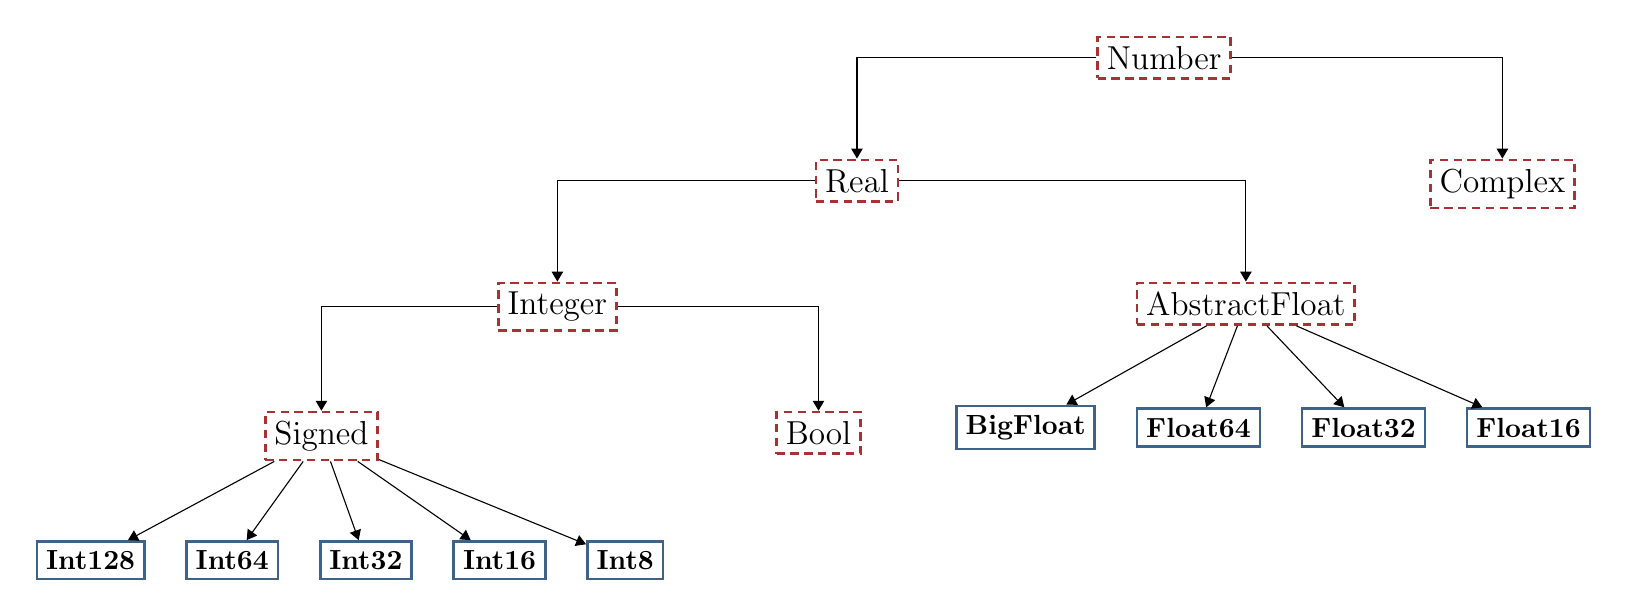
\begin{tikzpicture}[
   every node/.style       = {font=\large},
    node distance            = 1cm and 2.5cm,
         concreteNode/.style = {rectangle, align=center, draw= myblue, line width=1, font=\bfseries},
         abstractNode/.style = {rectangle, draw=myred, align=center, line width=1, densely dashed},
         myarrow/.style      = {-Triangle}
]
    \node[abstractNode] (number) {Number};

    \node[abstractNode, below left=of number, yshift=0cm, xshift=-0.0cm] (real) {Real};
    \node[abstractNode, below right=of number, xshift=-0.0cm] (complex) {Complex};

    \draw[myarrow] (number)  -| (real);
    \draw[myarrow] (number)  -| (complex);

    
    \node[abstractNode, below right=of real, xshift=0.5cm] (abstractfloat) {AbstractFloat};
    \node[abstractNode, below left=of real, yshift=-0cm, xshift=-0cm] (integer) {Integer};

    
    \draw[myarrow] (real) -| (abstractfloat);
    \draw[myarrow] (real) -| (integer);

        \node[abstractNode, below left=of integer, xshift=1cm] (signed) {Signed};
    \node[abstractNode, below right=of integer, xshift=-0.5cm] (bool) {Bool};

        \draw[myarrow] (integer) -| (signed);
    \draw[myarrow] (integer) -| (bool);

    
    \node[concreteNode, below left=of signed, xshift=1cm] (int128) {Int128};
     \node[concreteNode, right=of int128, xshift=-2cm] (int64) {Int64};
    \node[concreteNode, right=of int64,xshift=-2cm] (int32) {Int32};
    \node[concreteNode, right=of int32,xshift=-2cm] (int16) {Int16};
    \node[concreteNode, right=of int16,xshift=-2cm] (int8) {Int8};

    
    \draw[myarrow] (signed) -- (int128);
    \draw[myarrow] (signed) -- (int64);
    \draw[myarrow] (signed) -- (int32);
    \draw[myarrow] (signed) -- (int16);
    \draw[myarrow] (signed) -- (int8);

    \node[concreteNode, below left=of abstractfloat, ,xshift=2cm] (bigfloat) {BigFloat};
    \node[concreteNode, right=of bigfloat,xshift=-2cm] (float64) {Float64};
    \node[concreteNode, right=of float64,xshift=-2cm] (float32) {Float32};
    \node[concreteNode, right=of float32,xshift=-2cm] (float16) {Float16};
    

    \draw[myarrow] (abstractfloat) -- (float64);
    \draw[myarrow] (abstractfloat) -- (float32);
    \draw[myarrow] (abstractfloat) -- (float16);
    \draw[myarrow] (abstractfloat) -- (bigfloat);


\usetikzlibrary{calc}
\pgftransformreset
\node[inner sep=0pt,outer sep=0pt,minimum size=0pt,line width=0pt,text width=0pt,text height=0pt] at (current bounding box) {};
%add border to avoid cropping by pdflibnet
\foreach \border in {0.1}
  \useasboundingbox (current bounding box.south west)+(-\border,-\border) rectangle (current bounding box.north east)+(\border,\border);
\newwrite\metadatafile
\immediate\openout\metadatafile=\jobname_BB.txt
\path
  let
    \p1=(current bounding box.south west),
    \p2=(current bounding box.north east)
  in
  node[inner sep=0pt,outer sep=0pt,minimum size=0pt,line width=0pt,text width=0pt,text height=0pt,draw=white] at (current bounding box) {
\immediate\write\metadatafile{\p1,\p2}
};
\immediate\closeout\metadatafile
\end{tikzpicture}
\end{document}

